\subsection{The Purpose of Neural Networks for Image Processing}

Neural networks for image processing are an attempt to recreate the visual system in animals, creating algorithmic analogies to the various physical neuronal pathways that are present in the image. Typically, there are many different parts of our visual system that we take for granted, such as the ability to see upside down and extrapolate from prior information. While seemingly intuitive, these are difficult feats to determine algorithmically in a mathematical function.

Using neural networks for image processing is an attempt to re-create the visual system by utilizing algorithmic analogies to the human brain. Subjectively, we take many different aspects of our visual system for granted, like the ability to extrapolate to new information, and understand intuitively the notions of size and scale not affecting the content of an image. However, these are extremely difficult to perform with hand-selected features. Neural networks remove the need to feature selection in images, which has made them a powerful tool in the image processing toolbox.

\begin{figure}[h!]
  \centering
  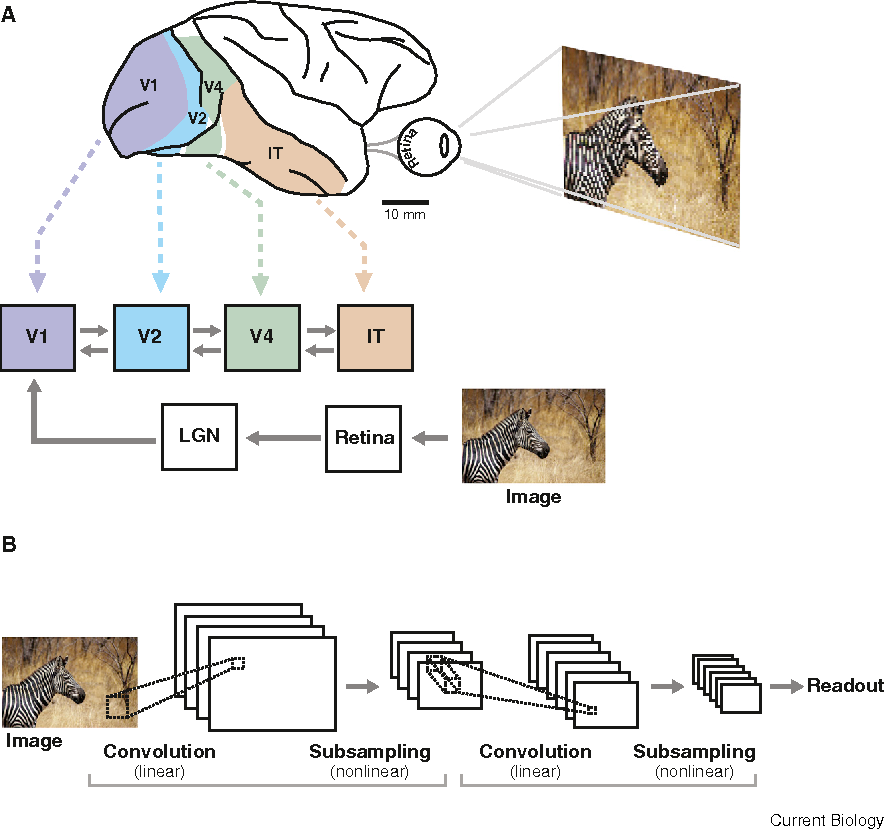
\includegraphics[width = 0.75\linewidth]{figures/raster/visual-nn.png}
  \caption{An example of a neural network mimicking the human brain.}
  \label{fig:nn-purpose-zebra}
\end{figure}

%%% Local Variables:
%%% mode: latex
%%% TeX-master: "../../../Jensen-Lit-Review"
%%% End:
